\chapter{Ion Scattering Methods}
There are a wide number of other important methods in surface science and it is beyond the scope of these notes to treat them all. Nevertheless the ion scattering methods deserve to be mentioned briefly since they are used widely and will be encountered quite often in the literature.

Previously we have seen how heavy ions like Ar could be used to remove atoms from the surface and how that combined with an analytical method like AES could be utilised to get information from deeper lying layers. In the following section we shall see how primarily light ions such as \ce{H+} or \ce{He+} can be used to actually identify various elements at the surface (Ion Scattering Spectroscopy), and also how they in the high energy version can be used to make a non-destructive depth profile. Both methods come in more advanced version where also surface geometry can be investigated and serve as tool for structural investigations like LEED.

\section{Low Energy Ion Scattering Spectroscopy}
The principle of Low Energy Ion Scattering (LEIS) or just Ion Scattering Spectroscopy (ISS) is very simple and can be performed in many UHV chambers in its basic version. All that is required is an ion gun and a bipolar analyser so that the energy of positive ions instead of electrons can be measured in an angle resolved manner. Naturally the set-up can be more advanced by having a well focused ion source so that lateral resolution can be obtained or with a movable analyser so that the ions can be detected in various scattering geometries. In the following we will only consider the simple version where the angle between the analyser and the ion gun is fixed. The geometry is depicted in \autoref{fig:isssetup}.

\begin{figure}[h!]
	\begin{center}
	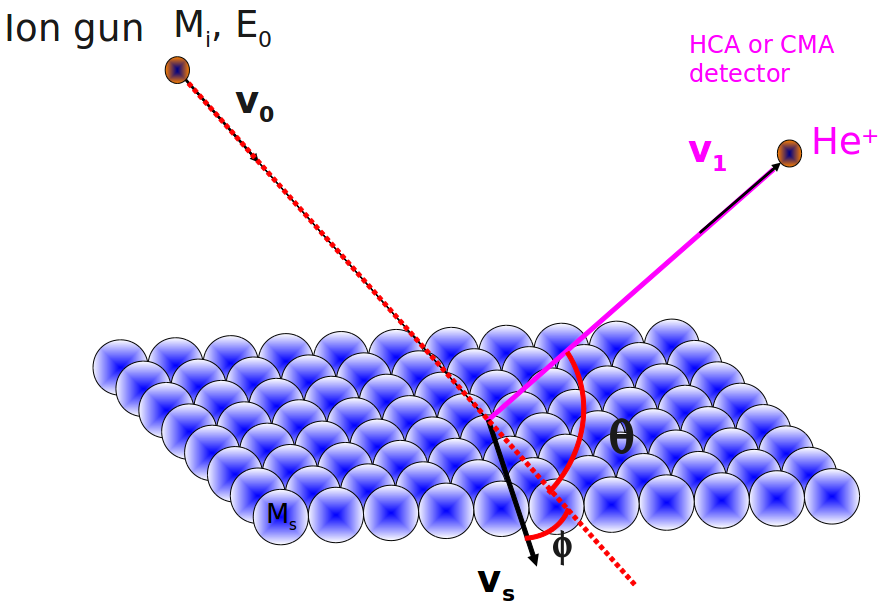
\includegraphics[scale=0.4]{figures/iss_ny_udg_11_01.png}
	\caption{Concept of the ISS set-up.}
	\label{fig:isssetup}
	\end{center}
\end{figure}

\begin{figure}[h!]
	\begin{center}
	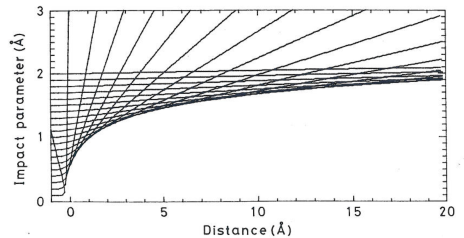
\includegraphics[scale=4]{figures/11_02.png}
	\caption{Calculated \ce{He+} ion trajectories as a function of impact parameter. The energy of the He beam was \SI{1}{k\electronvolt} and the target atom is Yb.}
	\label{fig:hetraject}
	\end{center}
\end{figure}

ISS usually refers to primary energies of \SIrange{1}{2}{k\electronvolt} energy of the ions. Preferentially He is used although heavier ions like Ne are also encountered. Very low ion doses are used in order not to create too much damage on the surface by sputtering processes. This is also one of the reasons for using lighter He ions. In this low  energy regime the ions interact almost perfectly through binary collisions with the surface atoms. The method is very surface sensitive since it has a large scattering cross section $\sim \si{\angstrom^2}$ and thereby a large shadow cone see \autoref{fig:hetraject} ensuring that most ions are not passing through the first layer of the sample. Furthermore most of the ions hitting the surface will be neutralised ($>\SI{99}{\percent}$) so very few of the particles survive the interaction as ions.

This makes the method particularly surface sensitive since ions which penetrates into the surface or undergoes multiple scattering processes will be neutralised and not detected in the electrostatic analyser if they were to be scattered back. Since it is a simple binary collision there will be conservation of momentum and energy:

\begin{equation}
M_i\vec{v_0}=M_i\vec{v_1}+M_s\vec{v_s}
\end{equation}

\noindent and
 
\begin{equation}
\frac{1}{2}M_iv_0^2=\frac{1}{2}M_iv_1^2+\frac{1}{2}M_sv_s^2
\end{equation}

\noindent where $M_i$ is the mass of the incoming ion, $M_s$ is the mass of the surface atom, $\vec{v_0}$ is the velocity of the incoming ion, $\vec{v_1}$ is the velocity of the scattered ion, and $\vec{v_s}$ is the velocity of the surface atom after the interaction.

After appropriate manipulation of the above equations the following ratio between the velocities of the incoming and outgoing ion can be found:

\begin{equation}
\frac{v_1}{v_0}=\frac{\pm\sqrt{M_s^2M_i^2\sin^2(\theta)}+M_i\cos(\theta)}{M_s+M_i}
\end{equation}

If the $M_i<M_s$ the plus sign applies and the ratio between the energy of the incoming and outgoing ion is:

\begin{equation}
\frac{E_1}{E_0}=\left[\frac{\sqrt{M_s^2-M_i^2\sin^2(\theta)}+M_i\cos(\theta)}{M_s+M_i}\right]^2
\end{equation}

The equation shows that the energy of the ion after the scattering event is only dependent on the initial energy of the ion, the angle $\theta$ and the mass of the surface atom. Since only the latter is unknown the mass of the surface atom can be determined. A typical ISS spectrum is shown in \autoref{fig:auruiss}.

\begin{figure}[h!]
	\begin{center}
	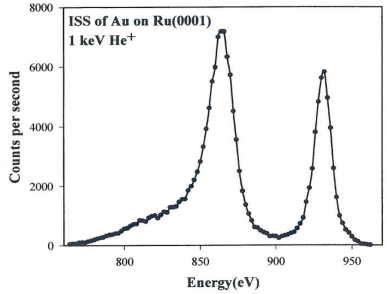
\includegraphics[scale=4]{figures/11_03.png}
	\caption{An ISS spectrum of Au deposited on a Ru(0001) single crystal. The primary ions were He+ at \SI{1000}{\electronvolt}.}
	\label{fig:auruiss}
	\end{center}
\end{figure}

The big advantage of ISS is that it is basically restricted to probing the surface layer. Thus if  say a 50-50 alloy is studied it is quite easily seen if one component segregates to the surface instead of the other one. The same results are in principle obtainable from an AES or XPS study, but here the deeper lying layers will always contribute as well which complicates the analysis. The mass resolutions are typically not very good (depends naturally on geometry and resolution power of the analyser) and it is usually not possible to distinguish two neighbour elements such as nickel and copper unless special equipment and isotopically cleaned samples are used. In some specific cases the resolution between different elements can be improved considerably by for instance using \ce{Ne+} ions instead of \ce{He+} ions, but great care should here be exercised that the surface is not damaged by sputtering during the measurements.

In dedicated instruments it may be possible to make angle resolved measurements changing the  angle of the analyser. By comparing such data to calculations of the absolute scattering cross section of the various atoms present on the surface and by making model calculations it is possible to extract information on the surface structure just as could be done by modelling LEED IV-curves. Such analysis is just as LEED restricted to well-behaved flat surfaces. Recently a dedicated instrument has been developed by \cite{Brongersma} utilising the advantages of the geometry of a CMA. By having the ion gun along the center of the analyser, which is normal to the surface, and collecting scattered ions in a ring  of the cylinder, a huge gain in signal can be obtained. This means that it first of all is very fast to perform an analysis and secondly only very small doses of ions are necessary limiting the potential danger of destruction of the surface.

\section{High Energy Ion Scattering Spectroscopy}
This method will only be treated briefly here since it is not a general method as it requires access to high energy accelerators. An extensive review of these methods can be found in \cite{feldman}. In a typical Rutherford Backscattering Spectroscopy (RBS) experiment ions are used which have energies in the range of \SIrange{0.5}{5}{M\electronvolt}. \ce{H+}, \ce{D+} and \ce{He++} ions at these energies have a very small cross section for scattering and will therefore have a penetration depth of several \si{\micro m} into the material. By measuring the energy of the ions scattered back - $\theta=\ang{170}$  - into a high energy ion detector it can in the same manner as for ISS be deduced which atoms the ion has encountered in the solid. The high energy ion detector is typically a gold coated silicon wafer where the ions during de-acceleration forms electron-hole pairs in the silicon in a number proportional to the energy of the incoming ion. Furthermore, as the ions will lose energy during penetration of the solid and since this energy loss can be estimated quite accurate is it possible to estimate the distance the ions have penetrated in the sample. An example of an RBS is shown in \autoref{fig:auruisstime} where \SI{3}{M\electronvolt} \ce{He+} ions are back scattered ($\theta=\ang{170}$) from a \SI{4000}{\angstrom} thick aluminium film with gold overlayers on both sides. Notice that the position of the front of the peaks reveals the element and the width the thickness of the various elements. Gold shows two peaks since ions scattered from the gold film on the back side will lose energy penetrating the aluminium film twice. Thus RBS analysis can be a powerful tool in many cases where it is necessary to analyse sandwich structures or diffusion profiles.

\begin{figure}[h!]
	\begin{center}
	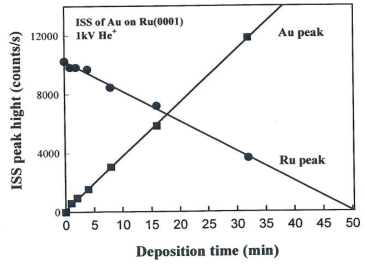
\includegraphics[scale=4]{figures/11_04.png}
	\caption{The ISS signals of Au and Ru as a function of Au deposition time.}
	\label{fig:auruisstime}
	\end{center}
\end{figure}

\section{Secondary Ion Mass Spectroscopy}
Secondary Ion Mass Spectroscopy (SIMS)is a method very similar to ISS in the sense that also here low energy ions are used and the conventional UHV equipment will be sufficient. But instead of performing energy analysis of the back scattered ions a mass analysis of particles sputtered away from the surface is performed as illustrated in \autoref{fig:alaubackscatter}. This allows for a detection of which elements, fractions of molecules, or clusters have been present on the surface. The method is very sensitive and can in some cases measure down to ppm levels of impurities in a sample. This makes the method particularly applicable in the microelectronic industry for characterizing for instance the silicon wafers for impurities and dopant.

\begin{figure}[h!]
	\begin{center}
	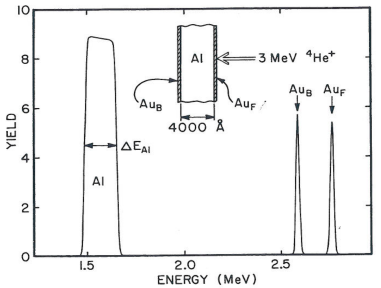
\includegraphics[scale=4]{figures/11_05.png}
	\caption{The back scattering spectrum of \SI{3.0}{M\electronvolt} He ions incident on a \SI{400}{\angstrom} aluminium film with thin gold marks on the front and the back \cite{feldman}.}
	\label{fig:alaubackscatter}
	\end{center}
\end{figure}

Quantitative analysis is in general difficult in surface science, but it is a particular problem in SIMS due to the fact that the method relies only on the ions coming off the surface. Ideally all species should be detected if a correct composition should be extracted. As we saw for the ISS experiments the chance of surviving as an ion was very little when interacting with the surface. Furthermore this probability will be very dependent on the element in question and the behaviour of the surface. In an approximate picture a simple relation can be obtained \cite{Norskovlang} where the probability for obtaining positive ions is given by

\begin{equation}
P^+\propto e^{-\dfrac{\Phi-A}{\epsilon_0}} 
\end{equation}

\noindent where $\Phi$ is the work function of the surface, $A$ is the affinity level of the atom leaving the surface and $\epsilon_0$ is a variable dependent, among other things, on the hopping matrix element of the electron from the atom to the surface and the velocity normal to the surface of the atom leaving. Similarly the probability for negative ions is given by

\begin{equation}
P^-\propto e^{-\dfrac{I-\Phi}{\epsilon_0}} 
\end{equation}

\noindent where $I$ is the ionisation potential of the atom leaving the surface. It is now obvious why the probability for obtaining signal in SIMS will vary orders of magnitude for the different elements and why it is not possible to say anything about the surface composition from a spectrum without taking the sensitivities of the different elements into consideration.  A SIMS spectrum of Si is shown in \autoref{fig:simsscheme} together with an AES analysis of the same surface. The SIMS analysis reveals many components which are not observed in the AES spectrum at all. That the probability also depends on the work function $\Phi$ makes things even worse since that will tend to vary strongly with the surface composition during a sputter profile.

\begin{figure}[h!]
	\begin{center}
	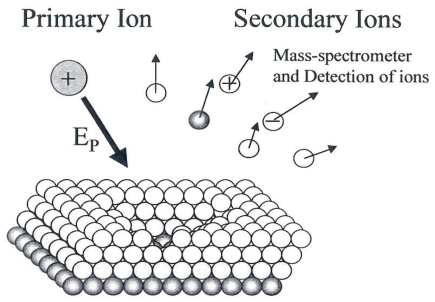
\includegraphics[scale=3]{figures/11_06.png}
	\caption{Schematic drawing of the SIMS process.}
	\label{fig:simsscheme}
	\end{center}
\end{figure}

The quantitative analysis can naturally be considerably improved by using well known standards and the method is particularly useful for measuring trace amounts of elements where methods like XPS and AES have to give in due to their detection limit (roughly 1 atomic percent). SIMS can also be used for measuring bigger fragments sputter off the surface. For instance SIMS has in some special cases been used in catalysis to monitor whether certain intermediates may be present at the surface or not. Even bigger fragments can be analysed, but then a conventional quadrupole mass spectrometer may not be sufficient any longer. Instead a Time of Flight  (TOF) technique is used. This approach is particular useful when analysing the fragments coming of polymer surfaces.

There are many interesting aspects to these ion based methods, but the reader is referred to Briggs and Seah for a thorough treatment \cite{briggs2} of this subject.